\subsection{Metric} 
%Semantic similarity of source code can be estimated via the similarity in term of different levels: lexical, syntax, and structural. Based on those three levels, we provide three metrics 

%\begin{table}
%\caption{Manual Semantic Score Criteria} 
%\begin{tabular}{|c|p{6.5cm}|}
%\hline
%Score & Description \\
%\hline
%0 & The translated method is totally incorrect and useless. One needs to rewrite the whole method. \\
%\hline
%1 & The translated method seems to be incorrect. Even though some parts are reusable, one is not willing to fix it and use the method. \\
%\hline
%2 &  It cannot be decided if the translated method is useful or not. \\
%\hline
%3 & The translated method seems to be correct. Even though it needs some adjustments, one is willing to reuse the method. \\
%\hline
%4 & The methods are identical in term of functionality. There is no change needed and it can be use as-is. \\
%\hline
%\end{tabular}
%\label{table:criteria}
%\end{table}

%Remind that our goal of the experiment is to (in)validate whether BLEU
%reflects the semantic accuracy of the migrated code from the tools
%with regard to the manual-migrated code in the ground truth. 
%
Remind that our goal of the experiment is to (in)validate whether BLEU
evaluates effectively the translated results based on the semantic accuracy 
of the migrated code from the tools with regard to the manual-migrated code 
in the ground truth. 
%
{\em Semantic accuracy} between the result from a SMT-based migration
tool and the reference code from the ground truth is the similarity
between their respective functionality. 
%
If two methods perform similar operations on the respective given
inputs, they are semantically similar, even interchangeable. A pair of
methods can have the same functionality despite of their difference in
term of code structure and code elements.
%
For example, a method using a \code{for} loop and another using a
\code{while} loop, they still can perform the same functionality even
though their lexical representations are much different. 
% Removed
%There exist many studies aiming to measure the functionality
%similarity of source code, which utilize the similarities of
%structures and
%dependencies~\cite{clone-tse07,roy09,baker97,ccfinder,cpminer,deckard,deckard2,horwitz01}.
%baxter98,ducasse99
%However, they are not reliable as their results sometimes contradict
%with human judgments on semantic accuracy~\cite{deckard2}. 
%
%More importantly, those structure-based metrics {\em do not reflect
%  human efforts} in fixing the incorrect migrated code into the
%correct one.
%
%Human judgment for our study would be the most reliable metric to
%measure semantic accuracy. 
% Tien
%To minimize the inaccuracy in evaluating similar functionality between
%the resulting code and the original code, 
To evaluate similar functionality between the translated code and the
original code, we adopted the same methodology as in the work by {\em
  Tsvetkov et al.}~\cite{tsvetkov-acl15} by using human judgment in
measuring semantic accuracy.
%Tien
%A human subject who examines a pair of methods can tell whether the
%code perform the same functionality.
%
% as well as explain the efforts needed
%in fixing the incorrectly migrated code into the correct one. 
%
Specifically, we conducted a study with human subject to manually
evaluate the migrated code from the SMT-based migration tools.
%2 goals

%Our study was conducted as follows:

\emph{1. Sample Size}. 
%
%Because our dataset contains a large number of pairs of code, it would
%take a lot of efforts to manually evaluate all of them. 
With our dataset containing 34,209 pairs translated methods, we aimed
to achieve the confidence level of 95\% and the margin of error of
5\%. Thus, according to CheckMarket~\cite{sample}, we randomly sampled
375 pairs of methods from the dataset for evaluation.

%According to~\cite{website}, from a population of 34,209, a sample
%size of 375 is acceptable with the confidence level of 95\% and the
%margin of error of 5\%. Therefore, we randomly sampled 375 pairs of
%methods from the dataset for evaluation.

\emph{2. Setting}. The human subject of our study is a developer who
is fluent and has more than 8 years of programming experience in both
Java and C\texttt{\#}. The evaluator is given each pair of methods in
C\texttt{\#}: one is the translated by a SMT tool and another one is
the reference code originally written by developers.
%
% (for example: a pair of method in figure xxx). Each method
%was labeled clearly as reference or machine-generated code.
(S)he was also given the original Java code to understand the
requirements of the migration task for this method. Moreover, (s)he
was provided with the Github links to the corresponding projects from
which those methods were extracted (with both Java and C\texttt{\#}
versions). This would give him/her a better context of the migrated
code.

\emph{3. Scoring.} The developer as the human subject was
told to give a score for each of 375 pairs of methods. The key
criteria in evaluating the migrated results is the semantic accuracy
with regard to the same functionality between the migrated code in
C\texttt{\#} and the original code in Java. 

If (s)he recognizes the same functionality between them, a perfect,
highest score of 4 must be given to the totally correct result. If
(s)he finds that the migrated code and the original one do not perform
the same functionality, a score of lower than 4 must be given
(inaccuracy). In this case of inaccurate results, we could ask the
evaluator to give a score to indicate the degree of semantic
inaccuracy. If so, the evaluator needs to quantify how close the
migrated methods in C\texttt{\#} are with respect to the functionality
of the respective methods in Java.  It is not straightforward to
provide a guideline for such quantification of the functional
similarities across several pairs of resulting code and original code.
%
On the other hand, the more the translated code functionally similar
to the original code, the more likely the users are willing to use the
translated code as the starting point for their migration task. That
is, the willingness to reuse the migrated code reflects its degree of
translation accuracy.
%
%However, it is a natural question to ask whether the developer is
%willing to reuse the not-quite-correct migrated code to start his/her
%migration process. That is, the willingness to reuse the migrated code
%reflects its degree of accuracy. 
%
Therefore, for the cases of inaccurate results, we chose to ask the
evaluator the questions relevant to the willingness to spend efforts
to reuse such results.

%
Particularly, if the migrated result was totally incorrect and (s)he
finds it totally useless and does not want to fix it, (s)he must give
a lowest score of 0 (\ie the migrated code is totally incorrect).
%
If (s)he is willing to fix the migrated code and reuse it, a score of
3 must be given (code seems to be not exactly correct, however, human
subject is willing to fix it). In contrast, if (s)he finds the
migrated code incorrect, and is not willing to reuse it, (s)he must
give a score of 1 (code seems to be incorrect in which some parts
could be reused). Finally, if the human subject is undecidable on
whether to reuse the migrated code, (s)he must give a neutral score of
2.

With this scheme, we are able to evaluate the quality of the migrated
code with the integration of both the semantic accuracy of the
resulting code with regard to the reference code in the ground truth,
and the willingness to correct the translated code to achieve the same
functionality as the original~code.

%We set two goals for the human subject in evaluating the results. The
%first goal is the correctness of the resulting code with respect to
%the manual-migrated code in the ground truth. The second one is based
%on the efforts needed to correct the translated code to achieve the
%same functionality as of the reference code in the ground truth.

%
%The scoring was based on the human efforts needed to fix the
%translated method to achieve the same functionality as of the
%reference one.

In summary, the score range is as follows:

\begin{compactitem}

\item {\bf Four}: A score of 4 means the pairs of methods are
  identical in term of functionality, and the translated method can be
  used as-is.

\item {\bf Three}: A score of 3 means the translated code seems to be
  correct. Even though it needs some minor modifications, one is
  willing to reuse the result.

\item {\bf Two}: A score of 2 means that the human subject cannot
  decide whether to reuse the translated code or not.

\item {\bf One}: A score of 1 means the translated code seems to be
  incorrect, and even though some parts of the result are reusable,
  one is {\em not} willing to fix the code.

\item {\bf Zero}: a score of 0 means the translated code is totally
  incorrect and useless, and it is better to re-write it entirely
  rather than reuse the result.

\end{compactitem}

%In short, the scoring guidelines are listed on
%Table~\ref{table:criteria}. 

% REMOVED
%Before actually giving the scores, the human subject could study our
%preselected examples with according scores and explanations. The
%examples are presented on Figure~\ref{fig:scoreEG}. Specifically, the
%code from line 11 to line 20 represents a result with a score of
%4. Noted that even though it is different from the reference code in
%term of actual program elements (use a regular \code{for} loop,
%instead of a \code{foreach}), it still performs the same
%functionality. A translated method of score 3 (lines 21 to line 30)
%seems to have similar functionality as the reference code, but it
%still needs minor editing (line 23 contains an incorrect function
%call, \code{indexOf} instead of \code{IndexOf} with an incorrect
%parameter). Lines 31 to 40 demonstrates a translated method which has
%score of 2. It cannot be decided if the method should be used or
%not. It has some good program elements that are similar to the
%reference code, but at the same time, has some critical errors that
%would be hard to fix. A translated method of score 1 (lines 41 to 50)
%has only one line of code that is reusable (line 43). So it is not
%worth fixing/reusing the code. Lines 51 to 60 represents a translated
%code of score 0 which means the entire translated code is totally
%useless, \ie it is better to rewrite the whole method.

%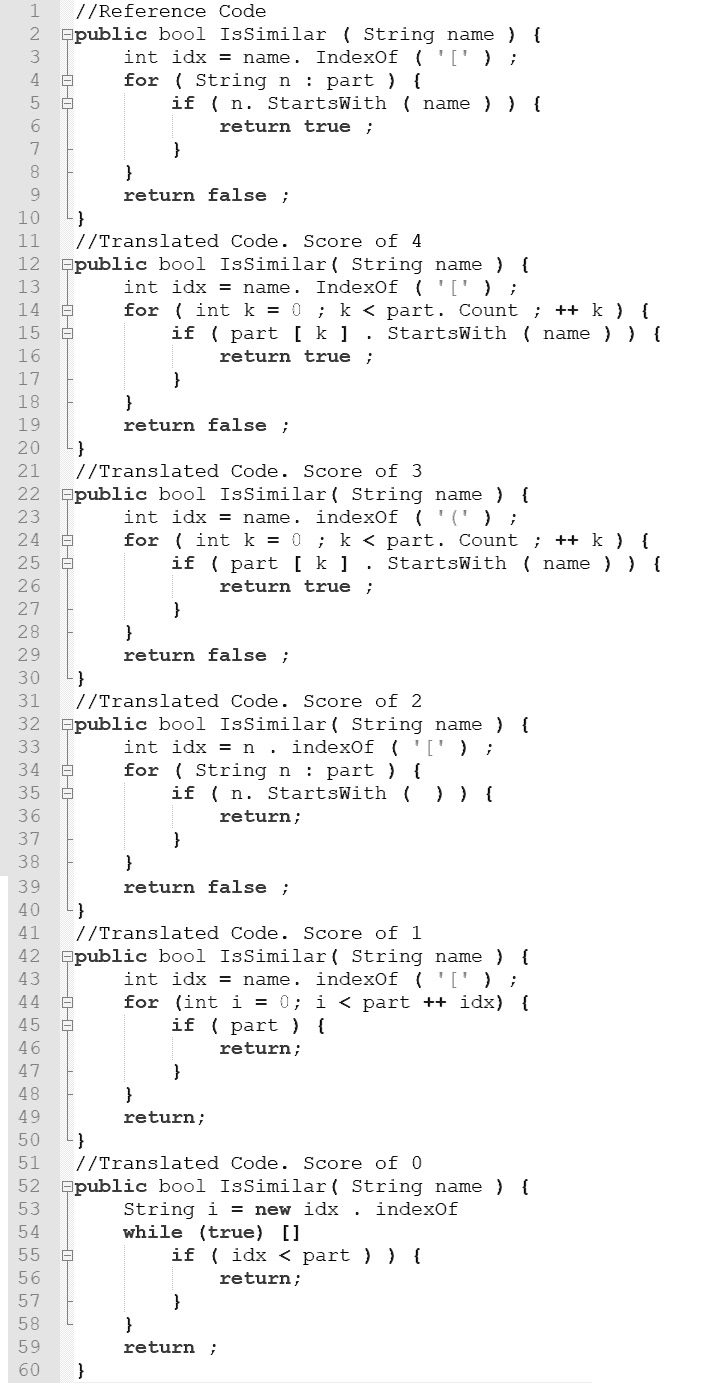
\includegraphics{scoreExamples}

We conducted the same human study for the translated results from all the above models. From now on, we regard those scores as \textbf{{\em
    semantic score}}.


%of both lpSMT and
%mppSMT models. As a result, we have scores for 375 pairs of methods
%for each model. From now on, we regard those scores as \textbf{{\em
%    Semantic score}}.

%\begin{figure}
%\caption{Scoring Examples}
%\centering
%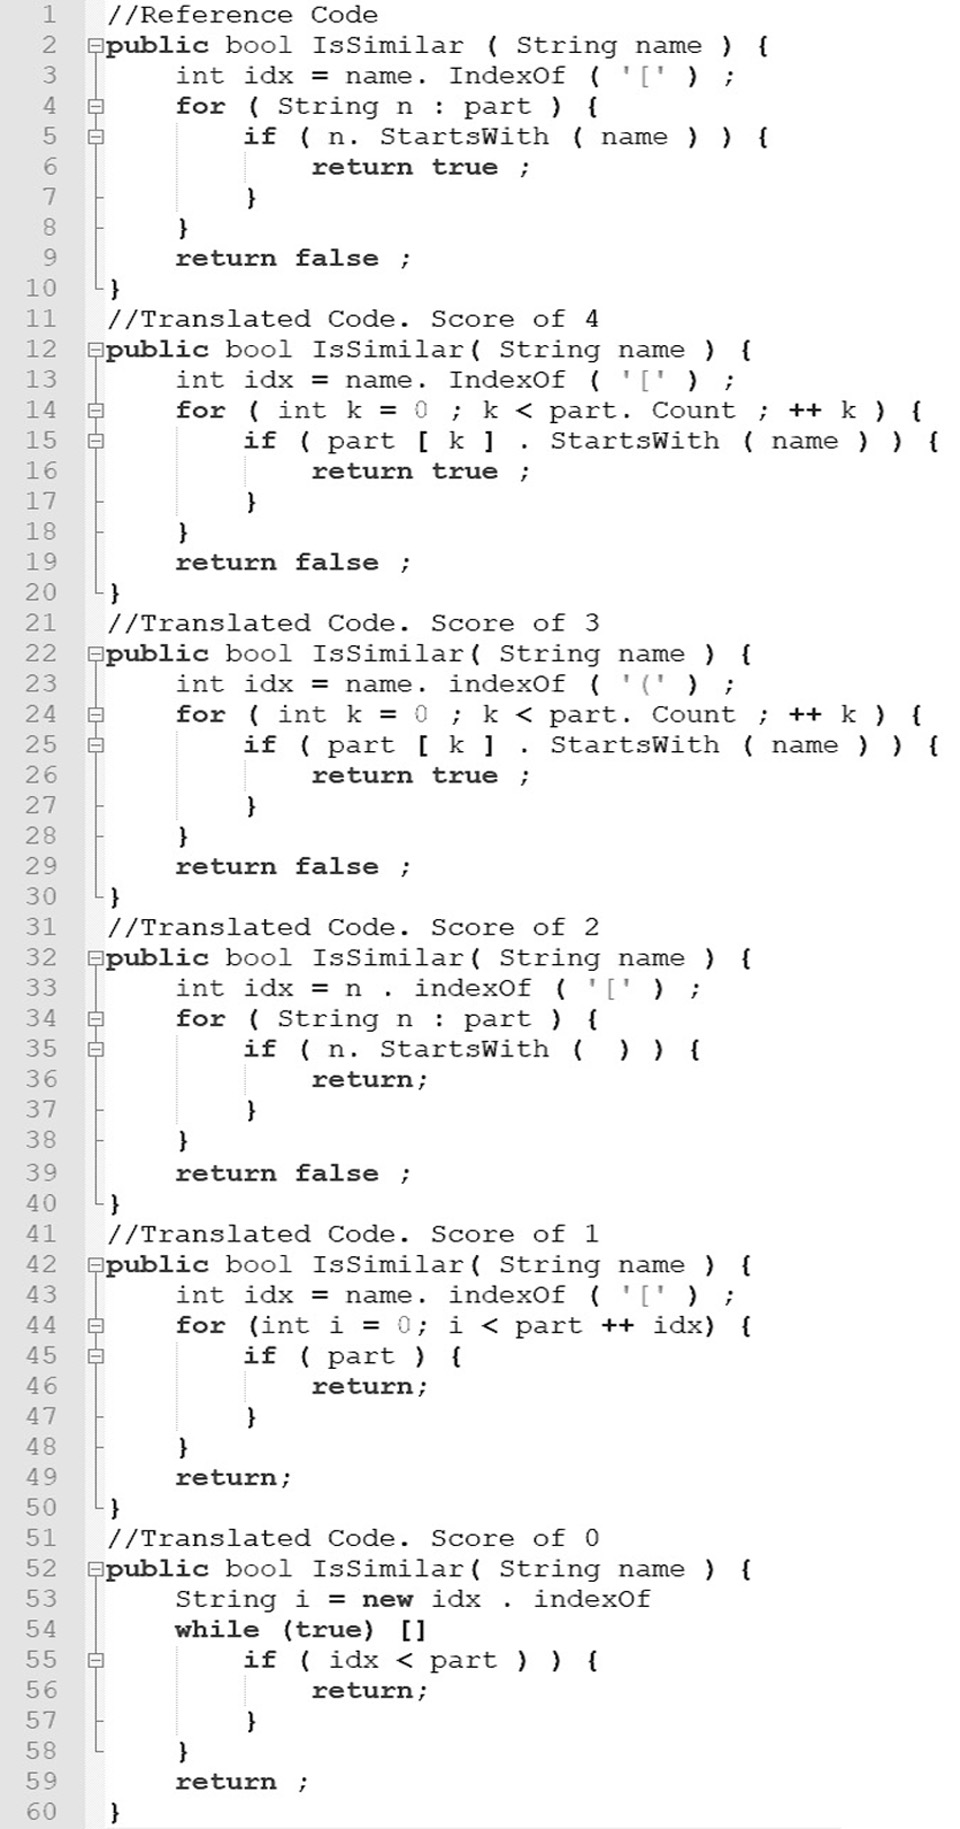
\includegraphics{img/scoreExamples}
%\label{fig:scoreEG}
%\end{figure}


%Our hypothesis states that \emph{\textit{BLEU score does not measure well the similarity in term of semantics between the reference and migrated source code}}. Therefore, given a pair of methods (reference one and machine translated one), we need a metric that can measure the similarity in term of semantics between them. As we know of, there is no automated metrics to do that task. To determine semantic similarity score, we used a human subject to manually evaluate pairs of methods to see how close they are in term of semantic/functionality. Specifically, scoring is done based on the human effort to fix the translated method to achieve the same functionality as of the reference one. The detailed scoring guidelines are presented in Table\ref{table:criteria}. The human subject is a senior developer who is fluent in both Java and C\#. He was given a pair of methods in C\# (machine generated one and reference one), the original method in Java, and the context project from which the methods come from. Then, he was told to evaluate pairs of methods in C\#, and give score as our guideline above and table \ref{table:criteria}. He could also refer back to the original Java method and project for a better understanding of the context. Below are examples for each score from -2 to 2:\\
%To determine semantic similarity score between pair of methods, we manually scored each pair from 0 to 6 based on the human effort to fix a translated method to a referenced one. Specifically, we list the criteria to score in Table  with a score of 0 means the pair of methods are totally different, and a score of 6 means they are totally the same. Scoring also follows the following principles: 1. An effort to fix a syntactical error (misplacing a semi-colon, parenthesis...) has less weight than an effort to fix a semantical error (wrong branch, wrong function call...). 2. A fix that requires adding sources code has more weight than one that requires removing/replacing. 3. A fix for user-defined program elements (identifier, simple name, method name) is more 'pricey' than a fix for keyword (this, if, for...). Example (of scores 1,3,5).

%Since our dataset contains a large number of pairs of methods, it would take a lot of efforts to manually evaluate all of them. Hence, we took a sample from our population of total 34,209 pairs. According to \cite{website}, our sample size is 375 with confidence level of $95\%$ and margin of error $5\%$. After we conducted the human experiment with 375 pairs of methods, we normalized the result on 0-1 range with 0 is respected to -2 and 1 is respected to 2.
